\documentclass{beamer}
%\usetheme{Singapore}
\usetheme{Darmstadt}
\useoutertheme{smoothtree}
\setbeamertemplate{footline}[page number]{}
\beamertemplateballitem
\usepackage{graphicx}
\usepackage{subfigure}
\usepackage{bm}
\usepackage{array,amsmath,latexsym,epsfig,float,afterpage,alltt,amssymb,theorem,enumerate,pstricks,bm,hhline,url,xr,float,multicol,multirow,ragged2e,colortbl,xspace, natbib}
\graphicspath{{figs/}}

\newcommand{\Blue}{\color{blue}}
\newcommand{\Red}{\color{red}}
\newcommand{\Green}{\color{green}}
\def\1{{\bf 1}}\def\rkhs{{\cal H}}

% Example definitions.
% --------------------

\def\cL{{\cal L}}
\def\cU{{\cal U}}
\def\cF{{\cal F}}
\def\cM{{\cal M}}
\def\cC{{\cal C}}
\def\cD{{\cal D}}
\def\cA{{\cal A}}


\def\bR{{\boldsymbol R}}
\def\bS{{\boldsymbol S}}
\def\bJ{{\boldsymbol J}}
\def\ba{{\boldsymbol a}}
\def\bb{{\boldsymbol b}}
\def\bw{{\boldsymbol w}}
\def\bu{{\boldsymbol u}}
\def\balpha{{\boldsymbol \alpha}}
\def\bbeta{{\boldsymbol \beta}}
\def\bd{{\boldsymbol d}}
\def\bb{{\boldsymbol b}}
\def\be{{\boldsymbol e}}
\def\bp{{\boldsymbol p}}
\def\bzero{{\boldsymbol 0}}
\def\bx{{\boldsymbol x}}
\def\by{{\boldsymbol y}}
\def\bv{{\boldsymbol v}}
\def\bq{{\boldsymbol q}}
\def\bxi{{\boldsymbol \xi}}
\def\liblinear{{{\sf LIBLINEAR}\xspace}}
\def\vw{{\sf VW}\xspace}
\def\pegasos{{\sf PEGASOS}\xspace}
\def\libsvm{{\sf LIBSVM}\xspace}

\def\bX{{\mathbf X}}
\def\x{{\mathbf x}}
\def\L{{\cal L}}

\AtBeginSubsection[]
{
    \begin{frame}<beamer>
        \frametitle{Outline}
        \tableofcontents[current,currentsubsection]
    \end{frame}
}


\begin{document}
\section{ }
\title[Machine Learning]{Machine Learning: Theory, Implementation and Practice}
\author[Ming-Hen Tsai]{
Ming-Hen (Henry) Tsai, \\
a Machine Learning Hacker for Good,
\url{scan33scan33@gmail.com}
}
\date{Jul 8, 2013}


%%-----------------------------------------------
%\begin{frame}
%\end{frame}


%-----------------------------------------------
\begin{frame}
\titlepage
\end{frame}

%%-----------------------------------------------
\begin{frame}{Outline}
\tableofcontents[pausesections]
\end{frame}

%-----------------------------------------------
\subsection{Introduction}

\begin{frame}
  \frametitle{What is Machine Learning?}
  \begin{itemize}
    \item Applications:
    \pause
    \item [] search engine, machine translation, spam filtering, medical imaging, etc.
    \pause
    \item In one sentence:
    \pause
    \item [] learning from {\it data}
    \pause
    \item How to learn?
    \pause
    \item [] {\it machine learning algorithms} learn a {\it model} from {\it data} 
  \end{itemize}
\end{frame}

\begin{frame}
  \frametitle{My View for Machine Learning}
  \begin{itemize}
    \item Machine Learning is a kind of data summarization technique that human can specify statistical rules in to get results to help people while leaving the judgment of results to the people.
    \pause
    \item It is not magic, we have to know something about the task.
    \pause
    \item It is usually constrained by the reach of human knowledge.
  \end{itemize}
\end{frame}

\subsection{Machine Learning Algorithms: Discriminative vs Generative Models with Sample Code}
\begin{frame}
  \frametitle{What are the machine learning algorithms out there?}
  \begin{itemize}
    \item Two types: generative model vs discriminative model
    \pause
    \item Generative: models that generate samples for a target task
    \item Discriminative: models that classify samples for a target task
    \pause
    \item {\bf End-to-end programs} below: random article generator (generative) and an audio classifier (discriminative).
  \end{itemize}
\end{frame}

\begin{frame}
  \frametitle{Random Article Generator -- Task Definition}
  \begin{itemize}
    \item From some article data, generate a new random article.
    \item Famous application: SCIgen by MIT.
  \end{itemize}
\end{frame} 

\begin{frame}
  \frametitle{Random Article Generator -- Model}
  \begin{itemize}
    \item First order hidden markov chain.
    \item Maintain a map keyed by word with its value as word-ratio pairs indicating how many times each word is next to the keyed word. (e.g. red $\to$ [(cat, 2), (dog, 3)])
    \item Beware of punctuations and special characters.
    \item Generation rule: given a word, randomly generate the next word weighed by word co-occurence.
    \item See {\scriptsize \url{https://github.com/scan33scan33/easyml/blob/master/text_generation/article_generator.py}} for 36 lines of code.
  \end{itemize}
\end{frame} 

\begin{frame}
  \frametitle{Audio Classification -- Task Definition}
  \begin{itemize}
    \item From some audio tracks some labeled positive and some labeled negative, train a model that tells positive ones from negative ones.
    \item Why? Audio format is something that is not semantically understandable. I want to write some simple programs to make it accessible.
  \end{itemize}
\end{frame} 

\begin{frame}
  \frametitle{Audio Classification -- Model}
  \begin{itemize}
    \item Record some audio tracks and do FFT.
    \item Use Perceptron to train a linear model.
    \item See {\scriptsize \url{https://github.com/scan33scan33/easyml/blob/master/voice_recognition/voice_auth.py}} for a few lines of code.
  \end{itemize}
\end{frame} 

\begin{frame}
  \frametitle{The Perceptron Algorithm}
  \begin{itemize}
    \item Input: $n$ training samples with labels $[(y_1, \bx_1), (y_2, \bx_2), \ldots, (y_n, \bx_n)]$.
    \item Output: a linear weight vector $\bw$.
    \item Algorithm Framework:
    \begin{enumerate}
    \item Initialize an initial $\bw = [0, \ldots, 0]$. 
    \item For each sample, $\bw \leftarrow \bw - (y_i - \text{sign}(\bw^T \bx_i)) \bx_i$.
    \end{enumerate}
  \end{itemize}
\end{frame} 

\subsection{Machine Learning Algorithms: from Theories to Packages}

\begin{frame}
  \frametitle{Some Theories}
  \begin{itemize}
    \item Statistical Theory: studies how generalized a model is
    \item Learning Theory: explains how algorithms work
    \item Psychology: studies how computer can simulate human beings (neural networks)
    \item Optimization Theory: makes algorithms run faster
  \end{itemize}
\end{frame} 

\begin{frame}
  \frametitle{Cores of Statistical Theory}
  \begin{itemize}
    \item Various statistical models (mostly on regression.)
    \item Each variable needs $k \ge 1$ samples to make it stable.
  \end{itemize}
\end{frame} 

\begin{frame}
  \frametitle{Cores of Learning Theory}
  \begin{itemize}
    \item Extensive analysis on classification models.
    \item VC-dimension (for classification): complex models have poor generalizability
    \item Learning models for simple algorithms: online-learning, PAC-learning, SQ, etc.
  \end{itemize}
\end{frame} 

\begin{frame}
  \frametitle{Cores of Optimization Theory}
  \begin{itemize}
    \item Hardness of the problem: $LP < QP < QCQP < SOCP < SDP$.
    \item CPU speed: $x$-GHz
    \item Memory access speed: DISK $\sim$ Network $<$ RAM $<$ Cache
    \item Example:
    \item [] 3-GHz CPU, 100 clocks for 1kB memory access and in avg 100 clocks per meta-instruction, linear time algorithm, 2GB data points in memory: $\frac{2 \times 100}{3} < 66 (\times \text{convergence iterations}) secs$
  \end{itemize}
\end{frame} 

\begin{frame}
  \frametitle{From Theories to Packages}
  \begin{itemize}
    \item Consider computer architecture: embedded, multi-core or distributed?
    \item Consider what algorithms to support.
    \item Write docs (or build a discussion group) for target users!!!
    \pause 
    \item [] Let's see some example packages.
  \end{itemize}
\end{frame}

\begin{frame}
\frametitle{LIBSVM}
\begin{itemize}
\item Optimized for multi-core architecture (using OPENMP). 
\item Linear to quadratic time algorithms to train non-linear models.
\item Linear convergence: $O(1/\epsilon)$
\end{itemize}
\end{frame}

\begin{frame}
\frametitle{LIBLINEAR}
\begin{itemize}
\item Optimized for multi-core architecture (using OPENMP). 
\item Linear time algorithms to train linear models.
\item Linear convergence: $O(1/\epsilon)$
\item Application to text classification: LIBSHORTTEXT.
\end{itemize}
\end{frame}

\begin{frame}
\frametitle{Take-home Message}
\begin{itemize}
\item Theories are mostly only for reference...
\item Good implementation can overcome theoretical difficulties...
\item But theoretical mindset is important.
\end{itemize}
\end{frame}

\subsection{Machine Learning: Real World Practice}
\begin{frame}
  \frametitle{A Real World Machine Learning System}
  \begin{figure}
  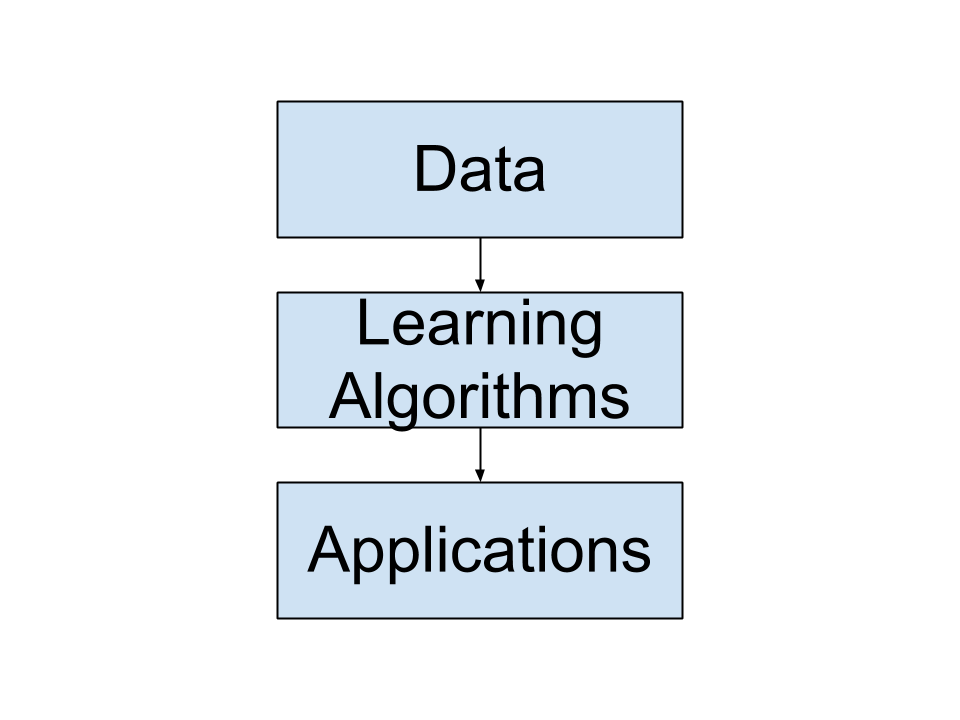
\includegraphics[width=4in]{Framework.png}\\
  \end{figure}
\end{frame}

\begin{frame}
  \frametitle{A Real World Machine Learning System with Industries}
  \begin{figure}
  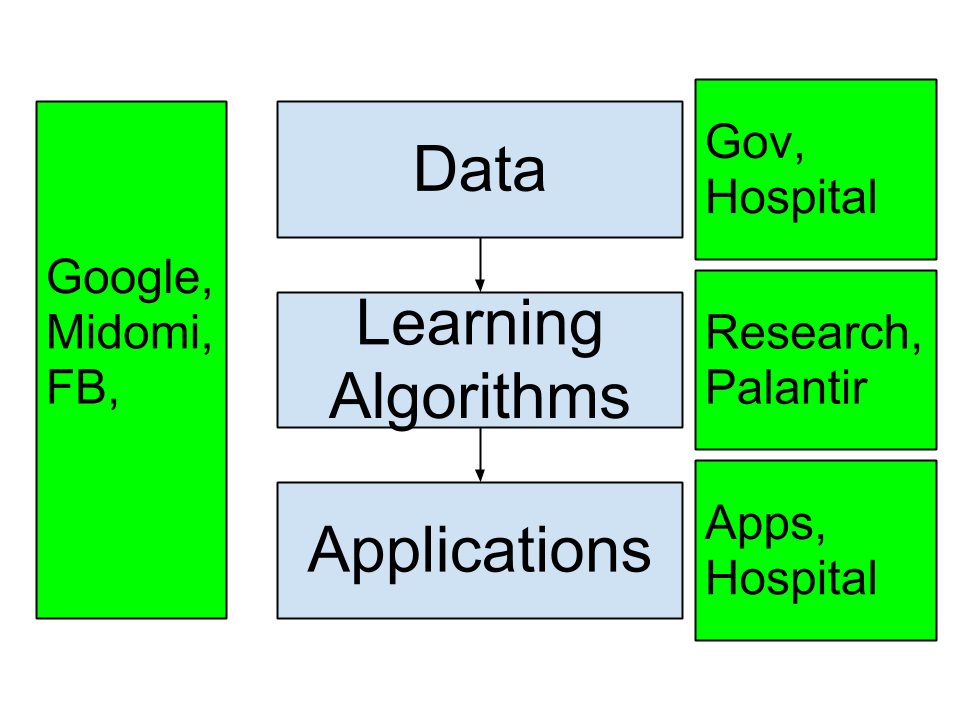
\includegraphics[width=4in]{Framework_Indus.png}\\
  \end{figure}
\end{frame}


\begin{frame}
  \frametitle{Challenges of Data Storage}
  \begin{itemize}
  \item Format: how to make other people access if needed 
  \item Fast data access: No-SQL, SQL vs files on disk...
  \item Privacy concerns
  \end{itemize}
\end{frame}

\begin{frame}
  \frametitle{Challenges of Model Complexity}
  \begin{itemize}
  \item Simple model: fast training/prediction time, accountable, saving computational power 
  \item Complex model: higher accuracy
  \end{itemize}
\end{frame}

\begin{frame}
  \frametitle{Good Models in Practice}
  \begin{itemize}
  \item Use meaningful features only
  \item Not sensitive to changes
  \end{itemize}
\end{frame}


\subsection{Review}
\begin{frame}
  \frametitle{Review}
  \begin{itemize}
  \item Machine learning: learning from data
  \item Give example codes for generative models and discriminative models
  \item Introduces some theories and how they are used in practice
  \item Connect all these to the industry needs
  \end{itemize}
\end{frame}

\begin{frame}
\frametitle{Code to infinity and beyond! Thanks!}

Thanks! The most update-to-date code and slides are at\\
	    \url{https://github.com/scan33scan33/easyml}.\\ 
\end{frame}


\end{document} 
